\documentclass[a4paper,11pt,article]{memoir}

\usepackage[a4paper,margin=1in]{geometry}

\usepackage[utf8]{inputenc}
\usepackage{fourier}
\usepackage{amsmath,amssymb}
\usepackage{graphicx}

\usepackage{color}
\definecolor{orange}{rgb}{0.75,0.5,0}
\definecolor{magenta}{rgb}{1,0,1}
\definecolor{cyan}{rgb}{0,1,1}
\definecolor{grey}{rgb}{0.25,0.25,0.25}
\newcommand{\outline}[1]{{\color{grey}{\scriptsize #1}}}
\newcommand{\revnote}[1]{{\color{red}\textit{\textbf{#1}}}}
\newcommand{\note}[1]{{\color{blue}\textit{\textbf{#1}}}}
\newcommand{\citenote}[1]{{\color{orange}{[\textit{\textbf{#1}}]}}}

\usepackage{xspace}

\usepackage{listings}
\usepackage{courier}
\lstset{basicstyle=\tiny\ttfamily,breaklines=true,language=Python}

\usepackage{fancyvrb}
\usepackage{url}

\usepackage{float}
\newfloat{listing}{tbp}{lop}
\floatname{listing}{Listing}

\title{GENIE GUI Design Notes}
\author{Ian~Ross}
\date{4 May 2015}

\begin{document}

\catcode`~=11    % Make tilde a normal character (danger of weirdness...)
%\catcode`~=13    % Make tilde an active character again

\tightlists

\maketitle

%======================================================================
\chapter{Use cases}

\subsection*{Completely new job}

\begin{itemize}
  \item{Create a new job in a selected job directory from a selected
    ``base'' and ``user'' configuration.}
  \item{Start job and monitor completion status.}
  \item{Post-process results.}
\end{itemize}

\subsection*{Modification of existing completed job}

\begin{itemize}
  \item{Clone an existing job configuration.}
  \item{Add parameter modifications on top of existing configuration.}
  \item{Start job and monitor completion status.}
  \item{Post-process results.}
\end{itemize}

\subsection*{Continuation from existing job}

\begin{itemize}
  \item{Clone an existing job configuration and set existing job as
    restart.}
  \item{Add parameter modifications on top of existing configuration.}
  \item{Start job and monitor completion status.}
  \item{Post-process results.}
\end{itemize}

\subsection*{Mid-job parameter modification}

\begin{itemize}
  \item{Pause an existing running job.}
  \item{Add parameter modifications on top of existing configuration.}
  \item{Restart job and monitor completion status.}
  \item{Post-process results.}
\end{itemize}

\subsection*{Cluster jobs}

\begin{itemize}
  \item{Create a job as usual.}
  \item{Run the job for a while to check for correctness.}
  \item{Pause the job.}
  \item{Submit job to cluster queue.}
\end{itemize}


%======================================================================
\chapter{Requirements}

%----------------------------------------------------------------------
\section{Basic functionality}

The idea here is to produce a simple GUI for configuring and managing
GENIE jobs.  It should allow a user to:
\begin{itemize}
  \item{quickly set up new jobs, either from scratch or based on
    existing jobs;}
  \item{start, stop and restart jobs;}
  \item{modify job parameters from the selected configuration
    (whatever that means in detail);}
  \item{monitor running jobs, both via the basic GENIE output and with
    real-time graphs of output variables;}
  \item{manage existing jobs: delete, rename, move, archive;}
  \item{access shared jobs (to clone or restart from existing shared
    experiments);}
  \item{manage job execution on clusters in a straightforward way.}
\end{itemize}

%----------------------------------------------------------------------
\section{Questions and possible answers}

\subsubsection*{How to manage communication between GUI and running jobs?}

GUI writes small command files into job directory; model looks for the
existence of a command file on each timestep.  Model writes response
into small response files that the GUI scans for periodically (for
running jobs).  Writing and reading small files avoids any issues with
file buffering.

There should probably be a configuration flag (\texttt{gui\_control}
in \texttt{data\_genie}?) to switch this functionality on and off --
jobs configured via the GUI can have this on.  (Alternatively, this
could be enabled all the time, which would allow the GUI to control
\emph{any} GENIE job...  I like that solution better.)

\subsubsection*{What happens when a job is stopped and restarted?}

\emph{Is it the same job as far as GENIE is concerned or should the
  GUI create a new copy of the job?} \\

When a job is stopped, the model writes restart files with names based
on the current timestep.  When a job is restarted, the GUI writes a
command file before starting the model that signals that a restart
from the latest available restart files is required.

This means that GUI jobs should always have all NetCDF restart file
generation options enabled -- job setup should override any such
options in the input configuration files to make sure that job pause
and restart works.

Alternatively, maybe it would be good to remove the options for
switching NetCDF restarts on and off and generate NetCDF restarts at
the end of \emph{every} job.  This would make it possible to continue
from the end of any job.

\subsubsection*{What happens to output files if a job is stopped and
  restarted?}

\emph{Does the model just append to the existing output files or
  should it start new ones?  What about if model parameters have been
  modified between stopping and restarting?} \\

If the model is just stopped and restarted via the GUI, the GUI will
write a command file to let the model know that it should restart from
the latest available restart.  In that case, all output files should
be opened for append, i.e. they should not be recreated, since the job
is just continuing from an earlier point.

Once a job has been started, the configuration is \emph{locked}.  This
means that you can't just stop a job, modify its configuration and
restart it.  You can instead create a new job to restart from the
existing job and modify \emph{its} configuration.

Alternatively, maybe it should be possible to modify the configuration
of \emph{any} stopped job, restarting as needed.  Configuration
modifications would then be saved with a time range for which they are
valid and graph views of model outputs would have annotations showing
when configuration options were changed.

\subsubsection*{How do cluster jobs work?}

Ideally, the GUI should detect whether or not it's running on the head
node of a cluster.  If it is, it ought to be possible to run jobs via
the cluster queuing system (so maybe there needs to be some sort of
GUI configuration options in \texttt{~/.cgenierc} to allow you to
specify the queue submission command?).

The way that this \emph{should} look is that a ``cluster job'' appears
to the user to be identical to a ``non-cluster job'', except that they
set a flag in the GUI saying that the job should be run through the
queuing system.  From an implementation perspective, the communication
between the GUI and the model should work just as for a job run on a
single node machine (assuming that the job directory is in the same
location on the cluster compute and head nodes, as is usually the
case, so that the GUI can write command files to the same location
independent of how the job is actually running).  One potential
problem is managing buffering of model output -- the GUI will need to
pick up model standard output and error streams from the output files
generated by the queuing system, and those streams need to be set up
to be unbuffered so that model output can be displayed in the GUI as
it appears.  (This is actually an issue for non-cluster jobs as well,
so maybe it just needs to be dealt with in a sensible way everywhere.
At the moment, for \texttt{gfortran}, I set the
\texttt{GFORTRAN\_UNBUFFERED\_PRECONNECTED} environment variable,
which ensures that standard output and standard error are unbuffered,
but maybe \emph{all} output streams should be set to unbuffered, using
the \texttt{GFORTRAN\_UNBUFFERED\_ALL} environment variable, because
this may be needed to ensure that time series output is flushed after
each timestep to allow for real-time plotting of values.  I need to
check though, because at least in BIOGEM, those time series files are
reopened, appended to and closed each timestep, so buffering ought not
to be an issue.  Needs investigation...)

%----------------------------------------------------------------------
\section{Job setup}

The notes in this and the following sections should be read in
conjunction with Figure~\ref{fig:job-life-cycle}, which shows the life
cycle of a job as managed by the GENIE GUI.  GUI buttons referred to
here can be seen in Figure~\ref{fig:gui-view-output}.

\begin{itemize}
  \item{New jobs are created by clicking on the ``New job'' button,
    and are initially created in an \textbf{UNCONFIGURED} state.
    Unconfigured jobs can be manipulated (moved, renamed, cloned,
    deleted, etc.) but cannot be run until the necessary configuration
    information is completed.}
  \item{For all job states except \textbf{RUNNING} and
    \textbf{ERRORED}, job configuration information can be edited
    under the ``Configuration'' tab in the GUI view.  For
    \textbf{UNCONFIGURED} jobs, the base and user configuration files
    can be selected.  For all editable job states, configuration
    ``modifications'' can be edited, as can the run length and the
    ``T100'' flag for the job.}
  \item{The full job configuration (i.e. the values that are used to
    generate the namelist files that GENIE reads at startup) is
    constructed from the base and user configuration files (as in the
    current system) plus superimposed ``modifications'' that allow for
    small changes to existing job configurations without the need to
    generate new base or user configuration files.  The idea here is
    to make it easy to set up and run variants of existing jobs.}
  \item{Job configuration ``modifications'' allow for changing both
    namelist parameters and forcing parameters.  (Not 100\% sure how
    to do this cleanly yet, but it's clearly needed.)}
  \item{Once an \textbf{UNCONFIGURED} job has had its configuration
    information set up, it becomes a \textbf{RUNNABLE} job.}
\end{itemize}

\begin{figure}
  \begin{center}
    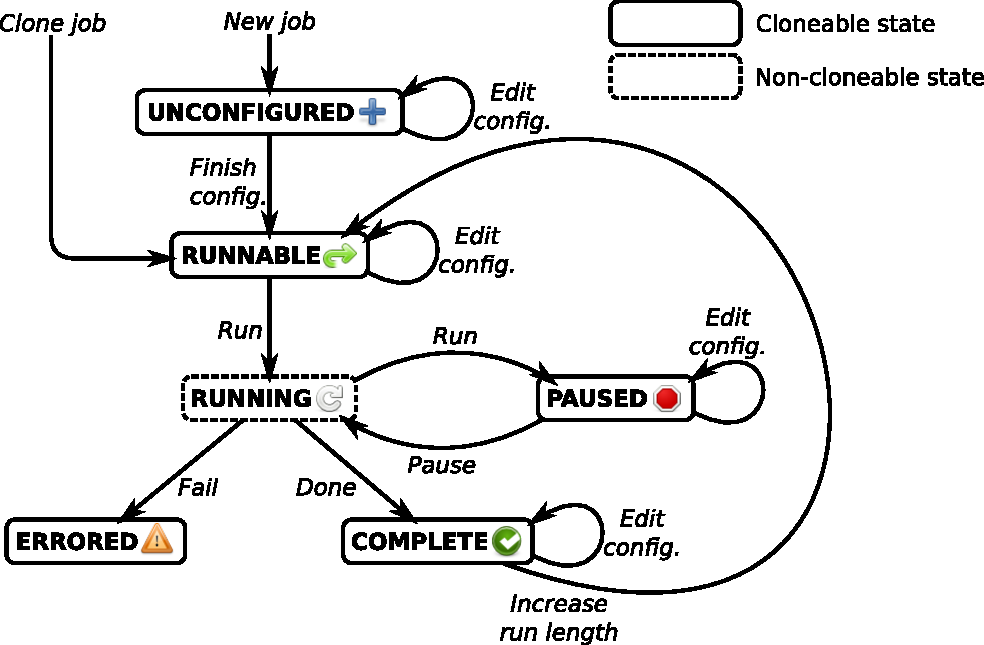
\includegraphics[width=0.8\textwidth]{job-life-cycle}
  \end{center}
  \caption{Life cycle of a job.  The icons for each job state are
    those used in the GUI -- see Figure~\ref{fig:gui-view-output}.}
  \label{fig:job-life-cycle}
\end{figure}

%----------------------------------------------------------------------
\section{Job control}

\begin{itemize}
  \item{\textbf{RUNNABLE} jobs can be started by pressing the ``Run
    job'' button in the GUI.  \textbf{RUNNING} jobs can be paused and
    restarted at will.}
  \item{Unless they are paused, \textbf{RUNNING} jobs run either to
    failure (in which case they become \textbf{ERRORED} jobs) or
    completion (\textbf{COMPLETE} jobs).}
  \item{It is possible to change the configuration of a job mid-run,
    either by pausing the job and editing its configuration
    information, or by editing the configuration information of a
    \textbf{COMPLETE} job and increasing its run length.  In this
    case, restarting the job creates a new ``run segment''.}
  \item{At the end of each run segment (i.e. when a job is paused or
    it completes), NetCDF restart files are written for each GENIE
    component so that a new run segment can be started from the end of
    the previous one.}
  \item{Each run segment has its own output log, which can be viewed
    in the ``Output'' tab of the GUI, and plots of model output data
    can span multiple run segments, with changes in model
    configuration marked on the plots.}
  \item{Model time series output for adjacent run segments where the
    model configuration has not changed are concatenated -- this makes
    it easy to simply run a job for a longer period than anticipated
    at its original setup if required.  Adjacent run segments with
    different model configurations have time series data stored in
    seperate files to avoid confusion, although GUI plots concatenate
    the data with indicators to show where model configuration
    information was changed.  (This approach is intended to make it
    easy to monitor jobs where instantaneous changes in forcing
    parameters are applied.)}
\end{itemize}

%----------------------------------------------------------------------
\section{Job monitoring}

\begin{itemize}
  \item{Model log output will be captured and displayed in a scrolling
    window under the ``Output'' tab in the GUI.  Model output
    buffering will be set up so that this output appears as the model
    runs to allow for real-time monitoring of the model state.}
  \item{For jobs with multiple ``run segments'' (i.e. jobs that have
    been paused and restarted, or restarted by extending their run
    length after they have completed), logs from previous run segments
    will also be saved and viewable.}
  \item{Real-time line plots of time series variables will be
    available under the ``Plots'' tabs (of which there can be more
    than one).}
  \item{Real-time plots will be zoomable and will show any number of
    selected variables on common axes.}
  \item{Plots for jobs with multiple run segments will indicate points
    in time where model configuration parameters changed.}
\end{itemize}


%======================================================================
\chapter{GUI layout}

\begin{description}
  \item[Job tree]{Multi-rooted tree, one root per top-level job
    directory in use (with options to add and remove additional job
    directories to view); hierarchical job sub-directories for
    organisation; leaf job directories marked with status icon (new
    and unconfigured, configured, running, complete, errored).}
  \item[Job actions]{Buttons and/or right-click menu in main job tree
    view:
    \begin{itemize}
      \item{Clone (available for all configured jobs);}
      \item{Move, delete, rename (all jobs);}
      \item{Archive (stopped/finished jobs);}
      \item{Run (configured/stopped jobs);}
      \item{Pause (running jobs);}
      \item{Submit to queue? (configured/stopped jobs).}
  \end{itemize}}
  \item[Configuration view]{Set and view base and user configuration
    files, run length, ``T100'' flag and restart information; view and
    edit ``modifications'' for both namelist variables and model
    forcing parameters; view resulting namelists and forcing data.}
  \item[Progress view]{View GENIE output in real-time (and output logs
    for completed model runs and ``run segments''); real-time graphing
    of selected model output (add/remove graph tabs, add/remove
    variables to plot in each tab); save selected graphs as ``preset''
    for later use.}
\end{description}

\begin{figure}
  \begin{center}
    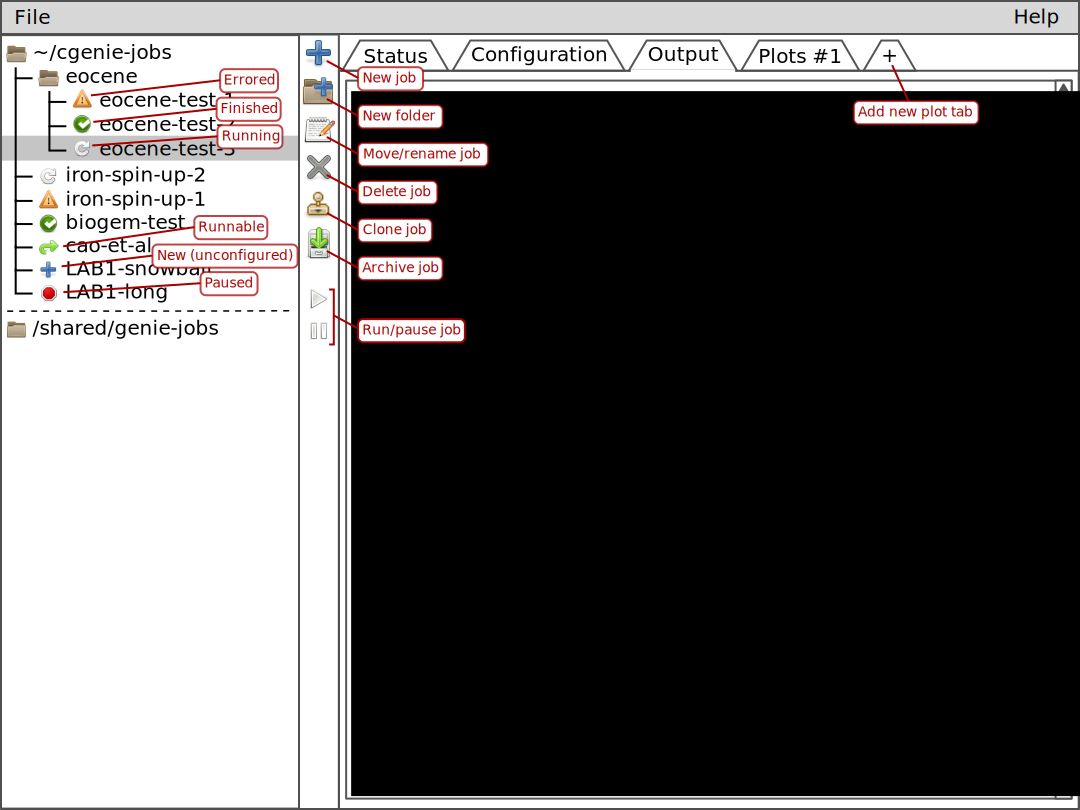
\includegraphics[width=\textwidth]{gui-view-output}
  \end{center}
  \caption{GUI layout: model output panel.}
  \label{fig:gui-view-output}
\end{figure}


%======================================================================
\chapter{Miscellaneous points}

\begin{itemize}
  \item{\textbf{All} GENIE jobs should write NetCDF restart files when
    they complete!}
  \item{Need to serialise state of job monitoring UI for use as
    ``presets'' in other jobs.}
  \item{Need reliable way to extract job status from jobs not managed
    by GUI (configured, running, finished).}
  \item{Need a way to pause and restart jobs -- pause needs to write a
    restart file to allow for restarting current job and generating
    new jobs from existing ones.}
\end{itemize}


%======================================================================
\newpage
\chapter{GENIE model changes}

%----------------------------------------------------------------------
\section{NetCDF restart generation}

Namelist variables controlling NetCDF restart generation are:
\begin{description}
  \item[\texttt{atchem}]{\texttt{par\_rstdir\_name="restart/atchem"}}
  \item[\texttt{atchem}]{\texttt{ctrl\_ncrst=.TRUE.}}
  \item[\texttt{atchem}]{\texttt{par\_ncrst\_name="\_restart.nc"}}

  \item[\texttt{biogem}]{\texttt{ctrl\_ocn\_rst\_reset\_T=.FALSE.}}
  \item[\texttt{biogem}]{\texttt{par\_rstdir\_name="restart/biogem"}}
  \item[\texttt{biogem}]{\texttt{ctrl\_ncrst=.TRUE.}}
  \item[\texttt{biogem}]{\texttt{par\_ncrst\_name="\_restart.nc"}}

  \item[\texttt{embm}]{\texttt{lout="rst"}}
  \item[\texttt{embm}]{\texttt{rstdir\_name="restart/embm"}}

  \item[\texttt{ents}]{\texttt{rstdir\_name="input/ents"}}

  \item[\texttt{goldstein}]{\texttt{rstdir\_name="restart/goldstein"}}
  \item[\texttt{goldstein}]{\texttt{lout="rst"}}
  \item[\texttt{goldstein}]{\texttt{rst\_reset\_T=.FALSE.}}

  \item[\texttt{goldsteinseaice}]{\texttt{rstdir\_name="restart/goldsteinseaice"}}
  \item[\texttt{goldsteinseaice}]{\texttt{lout="rst"}}

  \item[\texttt{sedgem}]{\texttt{par\_rstdir\_name="restart/sedgem"}}
  \item[\texttt{sedgem}]{\texttt{ctrl\_ncrst=.TRUE.}}
  \item[\texttt{sedgem}]{\texttt{par\_ncrst\_name="\_restart.nc"}}

  \item[\texttt{rokgem}]{\texttt{par\_rstdir\_name="restart/rokgem"}}
\end{description}

%======================================================================
\newpage
\chapter{Problems}

This is a (probably incomplete) list of problems with the GUI and the
interaction between the GUI and GENIE.

\begin{itemize}
  \item{When you pause and restart a job, the saving of BIOGEM time
    series data gets a bit screwed up, in the sense that there's a
    time shift between the model time and the time that BIOGEM thinks
    it should be writing output.  I spent a bit of time looking at
    this, but I think it's better for Andy to deal with it, probably
    as part of a general cleanup of time handling in the model, which
    is quite a mess.  There are probably the same kinds of problems in
    other forms of data output...}
\end{itemize}

\end{document}
